%---------------------- % % % Personnalisation des couleurs % % % ----------- MOUTARDE --------
\definecolor{couleurFonce}{RGB}{170,110,0} % Couleur du Code APOGEE
\definecolor{couleurClaire}{RGB}{222,190,137} % Couleur du fond de la bande
\definecolor{couleurTexte}{RGB}{255,255,255} % Couleur du texte de la bande
%------------------------------------------------------------------------------------------


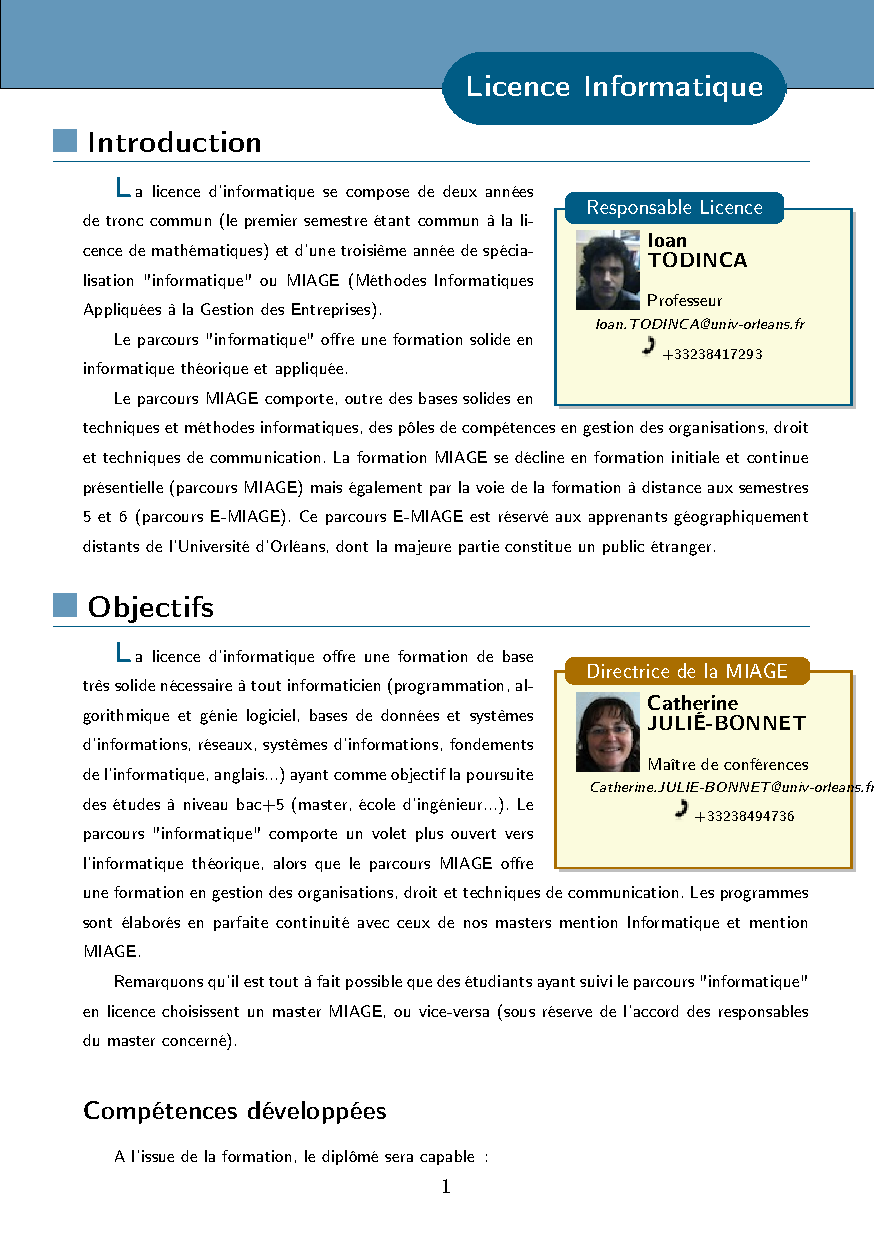
\includepdf[fitpaper,pages=-]{Preambule_Info_LicenceMIAGE_S5S6.pdf}

%==========================================================================================
% Semestre 5 : MIAGE
%==========================================================================================

\module[codeApogee={UE 51}, 
titre={Mise à niveau Informatique}, 
CODEUE={1}, 
COURS={}, 
TD={}, 
TP={12}, 
CTD={20}, 
TOTAL={32}, 
SEMESTRE={Semestre 5}, 
COEFF={0}, 
ECTS={0}, 
MethodeEval={Contrôle continue et terminal}, 
ModalitesCCSemestreUn={CC et CT}, 
ModalitesCCSemestreDeux={CT}, 
%CalculNFSessionUne={$\frac{(CC+2*CT)}{3}$}, 
%CalculNFSessionDeux={CT}, 
NoteEliminatoire={}, 
nomPremierResp={Catherine JULIÉ-BONNET}, 
emailPremierResp={Catherine.JULIE-BONNET@univ-orleans.fr}, 
nomSecondResp={}, 
emailSecondResp={}, 
langue={Français}, 
nbPrerequis={1}, 
descriptionCourte={true}, 
descriptionLongue={true}, 
objectifs={true}, 
ressources={true}, 
bibliographie={false}] 
{
Unité qui s\'intègre dans le PRL (Plan Réussite en Licence).\\
Obligatoire pour certains étudiants.
} 
{
Rappels sur l\'algorithmique et la programmation, les systèmes d\'exploitation, les outils de 
développement. 
} 
{Niveau bac + 2 en informatique ou équivalent} 
{\begin{itemize}
 \ObjItem Remise à niveau essentiellement destinée aux étudiants intégrant la Licence au semestre 5, afin de leur assurer les bases nécessaires pour suivre de manière satisfaisante les enseignements de troisième année.
\end{itemize} 
} 
{Ressources} 
{Biblio} 
 
\vfill

%==========================================================================================
\module[codeApogee={UE 52}, 
titre={Programmation avancée et structures dynamiques}, 
CODEUE={1}, 
COURS={20}, 
TD={30}, 
TP={}, 
CTD={}, 
TOTAL={50}, 
SEMESTRE={Semestre 5}, 
COEFF={4}, 
ECTS={4}, 
MethodeEval={Contrôle continue et terminal}, 
ModalitesCCSemestreUn={CC et CT}, 
ModalitesCCSemestreDeux={CT}, 
%CalculNFSessionUne={$\frac{(CC+2*CT)}{3}$}, 
%CalculNFSessionDeux={CT}, 
NoteEliminatoire={}, 
nomPremierResp={Jean-Jacques LACRAMPE}, 
emailPremierResp={Jean-Jacques.LACRAMPE@univ-orleans.fr}, 
nomSecondResp={}, 
emailSecondResp={}, 
langue={Français}, 
nbPrerequis={0}, 
descriptionCourte={true}, 
descriptionLongue={true}, 
objectifs={true}, 
ressources={true}, 
bibliographie={false}] 
{
Unité obligatoire. 
} 
{
Introduction au langage ADA. Types non contraints et pointeurs.
Unités de compilation, modularité, généricité.
Tâches, rendez-vous, type protégés, répartition.
Types étiquetés, programmation orientée objet, programmation par classe, héritage, héritage multiple. Interfaçage : autres langages, interface graphique, serveur web,... 
} 
{Maîtrise de l\'algorithmique de base (y compris les techniques d\'assertion et d\'invariant) et des structures statiques. Connaissance des principes de gestion mémoire, de la notion d\'état, de l\'affectation. Expérience des entrées sorties (non-)bufferisées. } 
{\begin{itemize}
 \ObjItem Acquérir et combiner plusieurs méthodes de programmation au sein d\'un même langage. Intégrer la notion d\'abstraction des données et des traitements. 
 \ObjItem Comprendre l\'intérêt du typage fort et de l\'induction de types. Arbitrer entre des solutions statiques et dynamiques. 
\end{itemize} 
} 
{Ressources} 
{Biblio} 
 
\vfill

%==========================================================================================
\module[codeApogee={UE 53}, 
titre={Réseaux}, 
CODEUE={1}, 
COURS={18}, 
TD={12}, 
TP={12}, 
CTD={}, 
TOTAL={42}, 
SEMESTRE={Semestre 5}, 
COEFF={4}, 
ECTS={4}, 
MethodeEval={Contrôle continue et terminal}, 
ModalitesCCSemestreUn={CC et CT}, 
ModalitesCCSemestreDeux={CT}, 
%CalculNFSessionUne={$\frac{(CC+2*CT)}{3}$}, 
%CalculNFSessionDeux={CT}, 
NoteEliminatoire={}, 
nomPremierResp={Abdelali ED-DBALI}, 
emailPremierResp={Abdelali.ED-DBALI@univ-orleans.fr}, 
nomSecondResp={}, 
emailSecondResp={}, 
langue={Français}, 
nbPrerequis={1}, 
descriptionCourte={true}, 
descriptionLongue={true}, 
objectifs={true}, 
ressources={true}, 
bibliographie={false}] 
{
Unité obligatoire. 
} 
{
Architecture des réseaux\,: structure en couches, protocoles, services. Réseaux locaux sous UDP-TCP/IP, Ethernet. Protocoles de routage\,: RIP, OSPF, BGP. Principaux protocoles Internet\,: DNS (annuaire de noms de domaines). SMTP (mail), FTP (transfert de fichiers), HTTP (web),... 
} 
{Algorithmique (modules de L1 et L2).} 
{\begin{itemize}
 \ObjItem Principes et pratique des réseaux locaux informatiques.
\end{itemize} 
} 
{Ressources} 
{Biblio} 
 
\vfill

%==========================================================================================
\module[codeApogee={UE 54}, 
titre={Analyse et conception des SI}, 
CODEUE={1}, 
COURS={20}, 
TD={20}, 
TP={10}, 
CTD={}, 
TOTAL={50}, 
SEMESTRE={Semestre 5}, 
COEFF={4}, 
ECTS={4}, 
MethodeEval={Contrôle continue et terminal}, 
ModalitesCCSemestreUn={CC et CT}, 
ModalitesCCSemestreDeux={CT}, 
%CalculNFSessionUne={$\frac{(CC+2*CT)}{3}$}, 
%CalculNFSessionDeux={CT}, 
NoteEliminatoire={}, 
nomPremierResp={Raymond RAKOTOZAFY}, 
emailPremierResp={Raymond.RAKOTOZAFY@univ-orleans.fr}, 
nomSecondResp={}, 
emailSecondResp={}, 
langue={Français}, 
nbPrerequis={0}, 
descriptionCourte={true}, 
descriptionLongue={true}, 
objectifs={true}, 
ressources={true}, 
bibliographie={false}] 
{
Unité obligatoire. 
} 
{
Contribution d\'une méthode d\'analyse et de conception, Merise en l\'occurrence, au sein des activités de l\'ingénierie des systèmes d\'information. Les principes généraux de la méthode. Le cycle d\'abstraction : raisonnements de modélisation et formalismes associés. Schémas des flux ; Modèle conceptuel des données (MCD) ; Modèle conceptuel des traitements (MCT) et modèle organisationnel des traitements (MOT). Le cycle de vie : la démarche. Étude préalable : Analyse de l\'existant et Conception du futur système ; Étude détaillée du futur système. 
} 
{} 
{\begin{itemize}
 \ObjItem Transformer les besoins et attentes des utilisateurs d\'un système d\'information en spécifications formalisées d\'une future application informatique.
\end{itemize} 
} 
{Ressources} 
{Biblio} 
 
\vfill

%==========================================================================================
\module[codeApogee={UE 55}, 
titre={Statistiques}, 
CODEUE={1}, 
COURS={}, 
TD={}, 
TP={30}, 
CTD={}, 
TOTAL={30}, 
SEMESTRE={Semestre 5}, 
COEFF={3}, 
ECTS={3}, 
MethodeEval={Contrôle continue et terminal}, 
ModalitesCCSemestreUn={CC et CT}, 
ModalitesCCSemestreDeux={CT}, 
%CalculNFSessionUne={$\frac{(CC+2*CT)}{3}$}, 
%CalculNFSessionDeux={CT}, 
NoteEliminatoire={}, 
nomPremierResp={Sophie JACQUOT}, 
emailPremierResp={Sophie.JACQUOT@univ-orleans.fr}, 
nomSecondResp={}, 
emailSecondResp={}, 
langue={Français}, 
nbPrerequis={1}, 
descriptionCourte={true}, 
descriptionLongue={true}, 
objectifs={true}, 
ressources={true}, 
bibliographie={false}] 
{
Unité obligatoire. 
} 
{
Statistique descriptive: cas uni et bidimensionnel. Statistique inférentielle\,: Démarche d\'échantillonnage: distribution d\'échantillonnage de la moyenne et de la variance dans le cas du tirage aléatoire.\,; Estimation paramètrique: qualités d\'une estimateur ponctuel, estimateur du maximum de vraisemblance, intervalle de confiance. Test: principes généraux des tests statistiques, tests de conformité, test d\'homogénéité, tests d\'ajustement, tests d\'indépendance. Étude des séries chronologiques: méthodes de filtrages (moyenne mobile, lissage exponentiel). Toutes les notions vues en cours sont illustrées en TP avec les logiciels R et XLSTAT. 
} 
{Notions de probabilités.} 
{\begin{itemize} 
 \ObjItem Le but du cours est de savoir mener une étude statistique sur des données avec un objectif précis. 
 \ObjItem Présentation synthétique des données, puis énoncé d\'hypothèses probabilistes et enfin validation de ces hypothèses, et enfin exploitation des résultats. 
\end{itemize} 
} 
{Ressources} 
{Biblio} 
 
\vfill

%==========================================================================================
\module[codeApogee={UE 56}, 
titre={Recherche Opérationnelle}, 
CODEUE={1}, 
COURS={16}, 
TD={24}, 
TP={}, 
CTD={}, 
TOTAL={40}, 
SEMESTRE={Semestre 5}, 
COEFF={3}, 
ECTS={3}, 
MethodeEval={Contrôle continue et terminal}, 
ModalitesCCSemestreUn={CC et CT}, 
ModalitesCCSemestreDeux={CT}, 
%CalculNFSessionUne={$\frac{(CC+2*CT)}{3}$}, 
%CalculNFSessionDeux={CT}, 
NoteEliminatoire={}, 
nomPremierResp={Prénom NOM}, 
emailPremierResp={Prenom.NOM@univ-orleans.fr}, 
nomSecondResp={}, 
emailSecondResp={}, 
langue={Français}, 
nbPrerequis={1}, 
descriptionCourte={true}, 
descriptionLongue={true}, 
objectifs={true}, 
ressources={true}, 
bibliographie={false}] 
{
Unité obligatoire. 
} 
{
Recherche opérationnelle sur les graphes : ordonnancement, flots. Programmation linéaire : méthode du simplex, dualité. 
} 
{algorithmique élémentaire sur les graphes} 
{\begin{itemize}
 \ObjItem Introduction à la recherche opérationnelle (modélisation et résolution).
\end{itemize} 
} 
{Ressources} 
{Biblio} 
 
\vfill

%==========================================================================================
\module[codeApogee={UE 57}, 
titre={Gestion comptable}, 
CODEUE={1}, 
COURS={30}, 
TD={}, 
TP={}, 
CTD={}, 
TOTAL={30}, 
SEMESTRE={Semestre 5}, 
COEFF={3}, 
ECTS={3}, 
MethodeEval={Contrôle continue et terminal}, 
ModalitesCCSemestreUn={CC et CT}, 
ModalitesCCSemestreDeux={CT}, 
%CalculNFSessionUne={$\frac{(CC+2*CT)}{3}$}, 
%CalculNFSessionDeux={CT}, 
NoteEliminatoire={}, 
nomPremierResp={Gilles LE FLOHIC}, 
emailPremierResp={Gilles.LE-FLOHIC@univ-orleans.fr}, 
nomSecondResp={}, 
emailSecondResp={}, 
langue={Français}, 
nbPrerequis={1}, 
descriptionCourte={true}, 
descriptionLongue={true}, 
objectifs={true}, 
ressources={true}, 
bibliographie={false}] 
{
Unité obligatoire. 
} 
{
Introduction\,: De la comptabilité générale à la comptabilité analytique. La détermination des coûts :
la méthode des coûts complets (Analyse des charges. Répartition des charges indirectes, enchaînements des calculs. Le coût de production.
Le coût de revient. La notion de résultat analytique d\'exploitation. Rapprochement avec la comptabilité générale. Critiques.)
Les méthodes des coûts partiels (Le coût variable ; le seuil de rentabilité. La méthode du coût indirect.
La méthode de l\'imputation rationnelle des charges fixes. Le coût marginal. ) Remise en cause des modèles traditionnels (La méthode ABC.).
} 
{Les notions de base en comptabilité financière, charges, bilan et compte de résultat.} 
{\begin{itemize}
 \ObjItem être capable de déterminer un coût. Réfléchir à la notion de prix, aux outils d\'aide à la décision.
\end{itemize} 
} 
{Ressources} 
{Biblio} 
 
\vfill

%==========================================================================================
\module[codeApogee={UE 58}, 
titre={Anglais}, 
CODEUE={1}, 
COURS={}, 
TD={24}, 
TP={}, 
CTD={}, 
TOTAL={24}, 
SEMESTRE={Semestre 5}, 
COEFF={2}, 
ECTS={2}, 
MethodeEval={Contrôle continue et terminal}, 
ModalitesCCSemestreUn={CC et CT}, 
ModalitesCCSemestreDeux={CT}, 
%CalculNFSessionUne={$\frac{(CC+2*CT)}{3}$}, 
%CalculNFSessionDeux={CT}, 
NoteEliminatoire={}, 
nomPremierResp={Marie-Françoise TASSARD}, 
emailPremierResp={Marie-Françoise.TASSARD@univ-orleans.fr}, 
nomSecondResp={}, 
emailSecondResp={}, 
langue={Français}, 
nbPrerequis={1}, 
descriptionCourte={true}, 
descriptionLongue={true}, 
objectifs={true}, 
ressources={true}, 
bibliographie={false}] 
{
Unité obligatoire. 
} 
{
\begin{itemize} 
 \item Restituer, échanger des informations, produire des énoncés corrects à l\'oral comme à l\'écrit.
 \item Travail personnel : Exercices d\'application à la fin de chaque unité et remise d\'un devoir au cours du semestre (CV).
 \item Travail individuel de remise à niveau en centre ressource multimédia si nécessaire.
\end{itemize} 
} 
{Avoir suivi avec succès les enseignements des semestres précédents.
} 
{\begin{itemize} 
 \ObjItem Comprendre et s\'exprimer dans une langue simple et correcte à l\'oral comme à l\'écrit afin d\'acquérir une autonomie suffisante dans le milieu professionnel
 \ObjItem Aide à la rédaction de CV et lettres de motivation dans le cadre de la recherche de stage.
\end{itemize} 
} 
{Ressources} 
{Biblio} 
 
\vfill

%==========================================================================================
\module[codeApogee={UE 59}, 
titre={Techniques de communication}, 
CODEUE={1}, 
COURS={}, 
TD={24}, 
TP={}, 
CTD={}, 
TOTAL={24}, 
SEMESTRE={Semestre 5}, 
COEFF={2}, 
ECTS={2}, 
MethodeEval={Contrôle continue et terminal}, 
ModalitesCCSemestreUn={CC et CT}, 
ModalitesCCSemestreDeux={CT}, 
%CalculNFSessionUne={$\frac{(CC+2*CT)}{3}$}, 
%CalculNFSessionDeux={CT}, 
NoteEliminatoire={}, 
nomPremierResp={Alfred HITCHCOCK}, 
emailPremierResp={Alfred.HITCHCOCK@univ-orleans.fr}, 
nomSecondResp={}, 
emailSecondResp={}, 
langue={Français}, 
nbPrerequis={1}, 
descriptionCourte={true}, 
descriptionLongue={true}, 
objectifs={true}, 
ressources={true}, 
bibliographie={false}] 
{
Unité obligatoire. 
} 
{
\begin{itemize} 
 \item Prise de parole devant un groupe : constituer et présenter un dossier avec documents.
 \item Travail de groupe et créativité : s\'initier aux méthodes de l\'invention pour innover dans un travail de groupe.
 \item Communication et programmation neurolinguistique (PLN) : se connaître, connaître autrui pour mieux communiquer.
 \item La recherche d\'emploi : le C.V., la lettre de motivation.
 \item Les écrits professionnels :
  \begin{itemize} 
    \item La lettre : lisibilité et créativité. La note de service : concision et précision.
    \item Le journal d\'entreprise : accroche et information.
    \item Le compte-rendu : recherche de l\'objectivité.
    \item Le rapport : aide à la prise de décision. 
  \end{itemize} 
\end{itemize} 
} 
{Savoir adapter un langage aux situations professionnelles.
} 
{\begin{itemize} 
 \ObjItem Savoir animer une réunion, connaître la communication orale professionnelle et rédiger des écrits professionnels en entreprise. 
\end{itemize} 
} 
{Ressources} 
{Biblio} 
 
\vfill

%==========================================================================================
\module[codeApogee={UE 60}, 
titre={Projet informatique}, 
CODEUE={1}, 
COURS={}, 
TD={6}, 
TP={}, 
CTD={}, 
TOTAL={6}, 
SEMESTRE={Semestre 5}, 
COEFF={3}, 
ECTS={3}, 
%MethodeEval={Contrôle continue et terminal}, 
ModalitesCCSemestreUn={Rapport et soutenance de projet}, 
ModalitesCCSemestreDeux={Pas de 2nde session}, 
%CalculNFSessionUne={$\frac{(CC+2*CT)}{3}$}, 
%CalculNFSessionDeux={CT}, 
NoteEliminatoire={}, 
nomPremierResp={Raymond RAKOTOZAFY}, 
emailPremierResp={Raymond.RAKOTOZAFY@univ-orleans.fr}, 
nomSecondResp={}, 
emailSecondResp={}, 
langue={Français}, 
nbPrerequis={0}, 
descriptionCourte={true}, 
descriptionLongue={true}, 
objectifs={true}, 
ressources={true}, 
bibliographie={false}] 
{
Unité obligatoire. 
} 
{
Projet de fin d\'études, faisant intervenir différentes connaissances et compétences acquises lors de l\'ensemble de la formation en licence.
} 
{Niveau de connaissance et de compétence de fin d\'année de licence (L3), en particulier dans les domaines de l\'analyse, de la modélisation et de la programmation.
Le langage de programmation souhaité pour le projet devra être connu ou maîtrisé dans un délai très court.
De plus il est obligatoire de s\'impliquer dans un groupe de travail et de posséder un minimum de qualités dans la communication.
} 
{\begin{itemize} 
 \ObjItem Au sein d\'un groupe, apprendre à organiser la réalisation complète d\'un projet, depuis l\'analyse jusqu\'aux tests de validation en utilisant des outils collaboratifs. 
 \ObjItem Percevoir les différentes compétences nécessaires au sein d\'un groupe de travail Se préparer au métier de chef de projet. 
\end{itemize} 
} 
{Ressources} 
{Biblio} 
 
\vfill

%==========================================================================================
\module[codeApogee={UE 60.1},
titre={Projet personnel et professionnel},
CODEUE={1},
COURS={12},
TD={12},
TP={},
CTD={},
TOTAL={20},
SEMESTRE={Semestre 5},
COEFF={2},
ECTS={2},
MethodeEval={Contrôle continue et terminal},
ModalitesCCSemestreUn={Production d\'un rapport},
ModalitesCCSemestreDeux={Production d\'un rapport},
%CalculNFSessionUne={$\frac{(CC+2*CT)}{3}$},
%CalculNFSessionDeux={CT},
NoteEliminatoire={},
nomPremierResp={Catherine JULIÉ-BONNET},
emailPremierResp={Catherine.JULIE-BONNE@univ-orleans.fr},
nomSecondResp={}, 
emailSecondResp={}, 
langue={Français}, 
nbPrerequis={0}, 
descriptionCourte={true}, 
descriptionLongue={true}, 
objectifs={true}, 
ressources={true}, 
bibliographie={false}] 
{
Unité obligatoire. 
} 
{
Préparation à la recherche de stage en entreprise. Techniques de communication dans le cadre professionnel, comportement et respect des règles de l\'entreprise et de la convention de stage.
Rédaction du rapport de stage et préparation d\'un exposé oral.
Présentation des différents types d\'emplois / métiers accessibles à l\'issue de la formation et des parcours de formation adéquats.
Étude d\'un projet professionnel personnel. 
} 
{} 
{\begin{itemize}
\ObjItem Se préparer au stage en entreprise, sur les plans législatif, comportemental et en terme de techniques de communication professionnelle. 
\ObjItem Connaître les différents types d\'emplois accessibles aux diplômés, les parcours de formation possibles, et commencer à cibler son propre projet professionnel et personnel.
\end{itemize} 
} 
{Ressources} 
{Biblio} 
 
\vfill

%==========================================================================================
% Semestre 6 : MIAGE
%==========================================================================================

\module[codeApogee={UE 61}, 
titre={Renforcement POO Java}, 
CODEUE={1}, 
COURS={}, 
TD={}, 
TP={12}, 
CTD={}, 
TOTAL={12}, 
SEMESTRE={Semestre 6}, 
COEFF={0}, 
ECTS={0}, 
MethodeEval={Contrôle continue et terminal}, 
ModalitesCCSemestreUn={CC et CT}, 
ModalitesCCSemestreDeux={CT}, 
%CalculNFSessionUne={$\frac{(CC+2*CT)}{3}$}, 
%CalculNFSessionDeux={CT}, 
NoteEliminatoire={}, 
nomPremierResp={Frédéric MOAL}, 
emailPremierResp={Frederic.MOAL@univ-orleans.fr}, 
nomSecondResp={}, 
emailSecondResp={}, 
langue={Français}, 
nbPrerequis={0}, 
descriptionCourte={true}, 
descriptionLongue={true}, 
objectifs={true}, 
ressources={true}, 
bibliographie={false}] 
{
Unité qui s\'intègre dans le PRL (Plan Réussite en Licence).\\
Obligatoire pour certains étudiants.
} 
{
Programmation orientée objet. Gestion de la mémoire. 
} 
{} 
{\begin{itemize}
  \ObjItem Assainir les lacunes encore présentes en programmation.
\end{itemize}
}
{Ressources} 
{Biblio} 
 
\vfill

%==========================================================================================
\module[codeApogee={UE 62}, 
titre={Génie Logiciel}, 
CODEUE={1}, 
COURS={12}, 
TD={20}, 
TP={8}, 
CTD={}, 
TOTAL={40}, 
SEMESTRE={Semestre 6}, 
COEFF={4}, 
ECTS={4}, 
MethodeEval={Contrôle continue et terminal}, 
ModalitesCCSemestreUn={CC et CT}, 
ModalitesCCSemestreDeux={CT}, 
%CalculNFSessionUne={$\frac{(CC+2*CT)}{3}$}, 
%CalculNFSessionDeux={CT}, 
NoteEliminatoire={}, 
nomPremierResp={Laure KAHLEM}, 
emailPremierResp={Laure.KAHLEM@univ-orleans.fr}, 
nomSecondResp={}, 
emailSecondResp={}, 
langue={Français}, 
nbPrerequis={1}, 
descriptionCourte={true}, 
descriptionLongue={true}, 
objectifs={true}, 
ressources={true}, 
bibliographie={false}] 
{
Unité obligatoire. 
} 
{
Généralités, cycle de vie d\'un logiciel, méthodes d\'analyse et de conception, méthodes objet, langage UML, méthodes de tests. 
} 
{notions de modélisation et de système d\'information} 
{\begin{itemize} 
 \ObjItem Acquérir une connaissance des outils et des techniques de spécification tels que les réseaux de Petri. 
 \ObjItem Maîtriser un langage dédié au génie logiciel, UML. 
\end{itemize} 
} 
{Ressources} 
{Biblio} 
 
\vfill

%==========================================================================================
\module[codeApogee={UE 63}, 
titre={Bases de données}, 
CODEUE={1}, 
COURS={12}, 
TD={20}, 
TP={8}, 
CTD={}, 
TOTAL={40}, 
SEMESTRE={Semestre 6}, 
COEFF={4}, 
ECTS={4}, 
MethodeEval={Contrôle continue et terminal}, 
ModalitesCCSemestreUn={CC et CT}, 
ModalitesCCSemestreDeux={CT}, 
%CalculNFSessionUne={$\frac{(CC+2*CT)}{3}$}, 
%CalculNFSessionDeux={CT}, 
NoteEliminatoire={}, 
nomPremierResp={Raymond RAKOTOZAFY}, 
emailPremierResp={Raymond.RAKOTOZAFY@univ-orleans.fr}, 
nomSecondResp={}, 
emailSecondResp={}, 
langue={Français}, 
nbPrerequis={1}, 
descriptionCourte={true}, 
descriptionLongue={true}, 
objectifs={true}, 
ressources={true}, 
bibliographie={false}] 
{
Unité obligatoire. 
} 
{
Algèbre relationnelle. SQL : Langage d\'Interrogation des Données. Dépendances fonctionnelles et Formes normales. SQL : Langage de Définition des Données. Mise en \oe uvre des contraintes d\'intégrité avec Oracle 
} 
{UE : Bases des données (L2).} 
{\begin{itemize} 
 \ObjItem Créer des bases de données relationnelles d\'une bonne forme normale. 
 \ObjItem Mettre en \oe uvre des contraintes d\'intégrité au sein de bases de données relationnelles. 
 \ObjItem Interroger des bases de données relationnelles. 
\end{itemize} 
} 
{Ressources} 
{Biblio} 
 
\vfill

%==========================================================================================
\module[codeApogee={UE 64}, 
titre={Programmation des SI}, 
CODEUE={1}, 
COURS={20}, 
TD={}, 
TP={20}, 
CTD={}, 
TOTAL={40}, 
SEMESTRE={Semestre 6}, 
COEFF={4}, 
ECTS={4}, 
MethodeEval={Contrôle continue et terminal}, 
ModalitesCCSemestreUn={CC et CT}, 
ModalitesCCSemestreDeux={CT}, 
%CalculNFSessionUne={$\frac{(CC+2*CT)}{3}$}, 
%CalculNFSessionDeux={CT}, 
NoteEliminatoire={}, 
nomPremierResp={Raymond RAKOTOZAFY}, 
emailPremierResp={Raymond.RAKOTOZAFY@univ-orleans.fr}, 
nomSecondResp={}, 
emailSecondResp={}, 
langue={Français}, 
nbPrerequis={1}, 
descriptionCourte={true}, 
descriptionLongue={true}, 
objectifs={true}, 
ressources={true}, 
bibliographie={false}] 
{
Unité obligatoire. 
} 
{
Contribution d\'une méthode de conception, Merise en l\'occurrence, au sein des activités de développement des systèmes d\'information. Architectures logicielles. Le cycle de vie, la démarche \,: Étude technique du futur système ; Production du logiciel et Déploiement. Le cycle d\'abstraction, raisonnements de modélisation et formalismes associés \,: Modèle logique des données (MLD)\,; Modèle physique des données (MPD) et modèle physique des traitements (MPT). Mise en \oe uvre d\'architecture logicielle en Développement Web. Mise en \oe uvre d\'activités de développement avec Oracle. 
} 
{} 
{\begin{itemize} 
 \ObjItem notion de modélisation, bases de données (niveau L2/L3) 
 \ObjItem Transformer des spécifications formalisées en une application informatique. 
\end{itemize} 
} 
{Ressources} 
{Biblio} 
 
\vfill

%==========================================================================================
\module[codeApogee={UE 65}, 
titre={Environnement économique de l\'entreprise}, 
CODEUE={1}, 
COURS={24}, 
TD={}, 
TP={}, 
CTD={}, 
TOTAL={24}, 
SEMESTRE={Semestre 6}, 
COEFF={3}, 
ECTS={3}, 
MethodeEval={Contrôle continue et terminal}, 
ModalitesCCSemestreUn={CC et CT}, 
ModalitesCCSemestreDeux={CT}, 
%CalculNFSessionUne={$\frac{(CC+2*CT)}{3}$}, 
%CalculNFSessionDeux={CT}, 
NoteEliminatoire={}, 
nomPremierResp={Gilles LE FLOHIC}, 
emailPremierResp={Gilles.LE-FLOHIC@univ-orleans.fr}, 
nomSecondResp={}, 
emailSecondResp={}, 
langue={Français}, 
nbPrerequis={0}, 
descriptionCourte={true}, 
descriptionLongue={true}, 
objectifs={true}, 
ressources={true}, 
bibliographie={false}] 
{
Unité obligatoire. 
} 
{
Les agents économiques et leurs fonctions. Keynes et les classiques : introduction a la macroéconomie. Le modèle is-lm. Emploi et chômage. Inflation et désinflation. État et politique économique. 
} 
{} 
{\begin{itemize} 
 \ObjItem Le cours vise à donner aux étudiants une information sur les thèmes essentiels de l\'économie contemporaine (chômage, inflation, politiques économiques,...) et à leur permettre d\'appréhender les principaux modes de raisonnement nécessaires à la compréhension de l\'environnement économique. 
 \ObjItem Pour ce faire, un retour théorique est opéré sur chaque thème, à partir d\'un regard sur l\'actualité conjoncturelle. 
\end{itemize} 
} 
{Ressources} 
{Biblio} 
 
\vfill

%==========================================================================================
\module[codeApogee={UE 66}, 
titre={Droit}, 
CODEUE={1}, 
COURS={24}, 
TD={}, 
TP={}, 
CTD={}, 
TOTAL={24}, 
SEMESTRE={Semestre 6}, 
COEFF={3}, 
ECTS={3}, 
MethodeEval={Contrôle continue et terminal}, 
ModalitesCCSemestreUn={CC et CT}, 
ModalitesCCSemestreDeux={CT}, 
%CalculNFSessionUne={$\frac{(CC+2*CT)}{3}$}, 
%CalculNFSessionDeux={CT}, 
NoteEliminatoire={}, 
nomPremierResp={Jean-Philippe CHALLINE}, 
emailPremierResp={Jean-Philippe.CHALLINE@univ-orleans.fr}, 
nomSecondResp={}, 
emailSecondResp={}, 
langue={Français}, 
nbPrerequis={0}, 
descriptionCourte={true}, 
descriptionLongue={true}, 
objectifs={true}, 
ressources={true}, 
bibliographie={false}] 
{
Unité obligatoire.
} 
{
Régime de protection juridique des logiciels et des produits informatiques. Droits de l\'auteur et de l\'utilisateur du logiciel. Fraude informatique. Loi informatique et Libertés. Contrats. 
} 
{} 
{\begin{itemize}
  \ObjItem Connaissance des droits et obligations de l\'utilisateur de produits informatiques, de l\'utilisateur d\'Internet et des mécanismes des contrats.
\end{itemize}
} 
{Ressources} 
{Biblio} 
 
\vfill

%==========================================================================================
\module[codeApogee={UE 67},
titre={Anglais},
CODEUE={1},
COURS={},
TD={25},
TP={},
CTD={},
TOTAL={25},
SEMESTRE={Semestre 6},
COEFF={3},
ECTS={3},
MethodeEval={Contrôle continue et terminal},
ModalitesCCSemestreUn={CC et CT},
ModalitesCCSemestreDeux={CT},
%CalculNFSessionUne={$\frac{(CC+2*CT)}{3}$},
%CalculNFSessionDeux={CT},
NoteEliminatoire={},
nomPremierResp={Marie-Françoise TASSARD}, 
emailPremierResp={Marie-Françoise.TASSARD@univ-orleans.fr}, 
nomSecondResp={},
emailSecondResp={},
langue={Français},
nbPrerequis={1},
descriptionCourte={true},
descriptionLongue={true},
objectifs={true},
ressources={true},
bibliographie={false}]
{
Unité obligatoire.
}
{
Travail de compréhension et d’expression à partir de documents authentiques longs et/ou complexes portant sur des innovations technologiques, des découvertes et avancées scientifiques.
} 
{Avoir suivi l\'unité "Anglais 5" ou un volume d\'heures de formation équivalente.} 
{\begin{itemize} 
 \ObjItem Comprendre l’information exprimée dans des messages complexes sur le domaine des Sciences et Technologies et s’exprimer sur ce même domaine à l’oral avec un degré suffisant de spontanéité et de fluidité (niveau européen\,: B2). 
\end{itemize} 
} 
{Ressources} 
{Biblio} 
 
\vfill

%==========================================================================================
\module[codeApogee={UE 68}, 
titre={Projet informatique}, 
CODEUE={1}, 
COURS={}, 
TD={}, 
TP={}, 
CTD={}, 
TOTAL={}, 
SEMESTRE={Semestre 6}, 
COEFF={3}, 
ECTS={3}, 
%MethodeEval={Contrôle continue et terminal}, 
ModalitesCCSemestreUn={Rapport et soutenance de projet}, 
ModalitesCCSemestreDeux={Pas de 2nde session}, 
%CalculNFSessionUne={$\frac{(CC+2*CT)}{3}$}, 
%CalculNFSessionDeux={CT}, 
NoteEliminatoire={}, 
nomPremierResp={Raymond RAKOTOZAFY}, 
emailPremierResp={Raymond.RAKOTOZAFY@univ-orleans.fr}, 
nomSecondResp={}, 
emailSecondResp={}, 
langue={Français}, 
nbPrerequis={1}, 
descriptionCourte={true}, 
descriptionLongue={true}, 
objectifs={true}, 
ressources={true}, 
bibliographie={false}] 
{
Unité obligatoire. 
} 
{
Réalisation d\'une application mettant en \oe uvre l\'analyse réalisée lors du projet de conception des SI. 
} 
{Unité "Programmation des systèmes d\'information".} 
{\begin{itemize} 
 \ObjItem Transformer des spécifications formalisées en une application informatique. 
 \ObjItem Rédiger des dossiers techniques : Dossier des Spécifications techniques, Dossier de programmation, Manuel Utilisateur.
\end{itemize} 
} 
{Ressources} 
{Biblio} 
 
\vfill

%==========================================================================================
\module[codeApogee={UE 69}, 
titre={Stage ou projet fin d\'études}, 
CODEUE={1}, 
COURS={}, 
TD={}, 
TP={}, 
CTD={}, 
TOTAL={0}, 
SEMESTRE={Semestre 6}, 
COEFF={6}, 
ECTS={6}, 
%MethodeEval={Contrôle continue et terminal}, 
ModalitesCCSemestreUn={Rapport et soutenance de stage ou de projet}, 
ModalitesCCSemestreDeux={Pas de 2nde session}, 
%CalculNFSessionUne={$\frac{(CC+2*CT)}{3}$}, 
%CalculNFSessionDeux={CT}, 
NoteEliminatoire={}, 
nomPremierResp={Frédéric MOAL}, 
emailPremierResp={Frederic.MOAL@univ-orleans.fr}, 
nomSecondResp={}, 
emailSecondResp={}, 
langue={Français}, 
nbPrerequis={1}, 
descriptionCourte={true}, 
descriptionLongue={true}, 
objectifs={true}, 
ressources={true}, 
bibliographie={false}] 
{
Unité obligatoire. 
} 
{
Stage d\'au moins trois mois consécutifs dans une entreprise ou projet de fin d\'étude, suivi par un enseignant et donnant lieu à la rédaction d\'un mémoire puis d\'une soutenance de stage en présence d\'un jury mixte d\'enseignants et de responsables de l\'entreprise. 
} 
{Compétences acquises au cours de la licence.} 
{\begin{itemize} 
 \ObjItem Capacité à participer et mener à bien un projet au sein d\'une entreprise. 
 \ObjItem Connaissance 
du monde professionnel.  
\end{itemize} 
} 
{Ressources} 
{Biblio} 
 
\vfill
